\documentclass[11pt]{article}
\usepackage[utf8]{inputenc} % Para caracteres en espa�ol
\usepackage{amsmath,amsthm,amsfonts,amssymb,amscd}
\usepackage{multirow,booktabs}
\usepackage[table]{xcolor}
\usepackage{fullpage}
\usepackage{lastpage}
\usepackage{enumitem}
\usepackage{multicol}
\usepackage{fancyhdr}
\usepackage{mathrsfs}
\usepackage{wrapfig}
\usepackage{setspace}
\usepackage{esvect}
\usepackage{calc}
\usepackage{multicol}
\usepackage{cancel}
\usepackage{graphicx}
\graphicspath{ {pictures/} }
\usepackage[retainorgcmds]{IEEEtrantools}
\usepackage[margin=3cm]{geometry}
\usepackage{amsmath}
\newlength{\tabcont}
\setlength{\parindent}{0.0in}
\setlength{\parskip}{0.05in}
\usepackage{empheq}
\usepackage{framed}
\usepackage[most]{tcolorbox}
\usepackage{xcolor}
\colorlet{shadecolor}{orange!15}
\parindent 0in
\parskip 12pt
\geometry{margin=1in, headsep=0.25in}
\theoremstyle{definition}
\newtheorem{defn}{Definition}
\newtheorem{reg}{Rule}
\newtheorem{exer}{Exercise}
\newtheorem{note}{Note}
\newcommand{\volume}{{\ooalign{\hfil$V$\hfil\cr\kern0.08em--\hfil\cr}}}
\newcommand{\parr}{\mathbin{\|}} % Parralel Symbol
\begin{document}
\setcounter{section}{3}
\setcounter{page}{38}
\setcounter{equation}{74}
%\definecolor{babyblue}{rgb}{0.54, 0.81, 0.94}
\definecolor{babyblueeyes}{rgb}{0.63, 0.79, 0.95}
\definecolor{babyblue}{rgb}{0.69, 0.88, 0.9}

 \pagestyle{fancy}
\fancyhf{}
\rhead{Section 2: Electromagnetics}
\rfoot{Page \thepage}
\thispagestyle{empty}


\begin{center}
{\LARGE \bf Section 2: Electromagnetics}\\
{\large AE435}\\
Spring 2018
\end{center}
In this section, we will review the basics of charge, electricity, magnetism, and Maxwell equations.
\vspace{5mm}
\section{Magnetostatics with Magnetic Media}
\begin{center}
\vspace{25mm}
\end{center}
\tableofcontents
\newpage
\subsection{Effect of Magnetic Media}
In our previous discussion, we only considered magnetostatics involving steady currents in a vacuum. Now we will examine...
\begin{itemize}
\item \textbf{Question: }What happens if matter is present?
\item \textbf{Answer: }The magnetic field $\vv{B}$ changes!
\item \textbf{Reason: }Matter has micro-currents associated with the motion of the electrons around atoms, "atomic currents"
\item \textbf{Aftermath: }So now we must consider two kinds of currents:
\begin{itemize}
\item Conduction currents, involving free charges
\item Atomic currents, with no charge transport (to the first order)
\end{itemize}
\end{itemize}
\newline
Each atom has a magnetic dipole moment.
\begin{shaded}
 \newline
 \textbf{Magnetic Dipole Moment}
\begin{equation}
\begin{aligned}
\vv{m}_i = \frac{1}{2} J_i \oint_c \vv{r}_i \times \mathrm{d}\vv{l}
\end{aligned}
\end{equation}
\end{shaded}
We can define a macroscopic vector quantity analogous to polarization, known as the \textbf{magnetization} or the magnetic dipole moment per unit volume. 
\begin{shaded}
 \newline
 \textbf{Magnetization}
\begin{equation}
\begin{aligned}
\vv{M} = \lim_{\Delta\volume\rightarrow0} \, \frac{1}{\Delta\volume} \, \sum_i \vv{m}_i
\end{aligned}
\end{equation}
\end{shaded}
In the \textbf{unmagnetized state}, $\vv{M}=0$ because $\vv{m}_i$ have random orientations that cancel out. In the presence of an external $\vv{B}$, matter becomes organized and $\vv{M}$ can become nonzero depending on the material properties. 
\newpage
\begin{center}
\vspace{1mm}
\end{center}
\textbf{Magnetization Current: }How does magnetization give rise to currents?
\begin{center}
\vspace{40mm}
\textbf{Figure 20}
\end{center}

For a uniform $\vv{M}$, currents cancel in the interior but not on the exterior. The result is a net surface current as shown in Figure 20. 
\newline
\newline
Similarly, if $\vv{M}$ is non-uniform, we can have an internal net current.
\newline
\newline
\newline
We can define a \textbf{Magnetization Current Density: }
\newline
\begin{equation}
\begin{aligned}
\vv{j}_m = \nabla \times \vv{M}
\end{aligned}
\end{equation}
\newpage
\subsection{Total Magnetic Field}
To incorporate $\vv{j}_m$ into Ampere's Law (Equation 72) we have to modify the magnetic field equations, just as we modified Gauss' law to include $\rho_e$. 
\newline
\newline
As before, we still have no monopoles:
\newline
\begin{equation*}
\begin{aligned}
\nabla \cdot \vv{B} = 0
\end{aligned}
\end{equation*}
But now, Ampere's law becomes:
\newline
\begin{equation}
\begin{aligned}
\nabla \times \vv{B} = \mu_o \, (\vv{j}+\vv{j}_m)
\end{aligned}
\end{equation}
Using Equation 77, we can write this as:
\begin{equation*}
\begin{aligned}
\nabla \times \bigg(\frac{1}{\mu_o}\,\vv{B}-\vv{M}\bigg) = \vv{j}
\end{aligned}
\end{equation*}
Where $(\frac{1}{\mu_o}\,\vv{B}-\vv{M})$ depends only on conduction current density $\vv{j}$ as its source. As a results, we define a vector field:
\begin{shaded}
 \newline
 \textbf{Magnetic Intensity or "H"-field}
 \newline
\begin{equation}
\begin{aligned}
\vv{H} = \frac{1}{\mu_o}\,\vv{B}-\vv{M} \qquad \bigg[\frac{\text{A}}{m}\bigg] = [\text{Oersted}]
\end{aligned}
\end{equation}
\newline
\textbf{Note:} 1 $\frac{\text{A}}{m}$ = 0.01257 Oersted
\end{shaded}
Finally, \textbf{Ampere's Law for Magnetic Media} is:
\newline
\begin{equation}
\begin{aligned}
\nabla \times \vv{H} = \vv{j}
\end{aligned}
\end{equation}
\newpage
A comparison of Magnetostatics and Electrostatics:
\setlength{\arrayrulewidth}{.5 mm}
\setlength{\tabcolsep}{18pt}
\renewcommand{\arraystretch}{2}
\begin{center}
 \begin{tabular}{| c | c |} 
 \hline
 \rowcolor{gray} \textbf{Electrostatics} & \textbf{Magnetostatics} \\ [1ex] 
 \hline
 \rowcolor{lightgray} In vacuum (no $\rho_p$) & In vacuum (no $\vv{j}_m$) \\  [1ex] 
 \hline
 $\nabla \cdot \vv{E} = \frac{q}{\epsilon_o} \quad$ (isolated charges) & $\nabla \cdot \vv{B} = 0$ \\ [1ex] 
 $\nabla \cdot \vv{E} = \frac{\rho_e(\vv{r})}{\epsilon_o} \quad$ (distributed charges) & \\ [1ex] 
 $\nabla \times \vv{E} = 0 & $\nabla \times \vv{B} = \mu_o \vv{j}$ \\ [1ex] 
  \hline
  \rowcolor{lightgray} With media effects (finite $\rho_p$) & With media effects (finite $\vv{j}_m$) \\ [0.5ex] 
 \hline
 $\nabla \cdot \vv{E} = (\rho_f + \rhp_p)/\epsilon_o$ & $\nabla \cdot \vv{B} = 0$ \\ [1ex] 
 $\nabla \cdot \vv{D} = \rho_f$                                   &  \\ [1ex] 
 $\nabla \times \vv{E} = 0$                                        & $\nabla \times \vv{B} = \mu_o (\vv{j}+\vv{j}_m)$ \\ [1ex] 
 & $\nabla \times \vv{H} = \vv{j}$ \\ [1ex] 
 \hline
 \end{tabular}
\end{center}
We can also derive the intergral equation for magnetic intensity. From Equation 80, if we integrate over a surface element and apply Stokes theorem on a closed curve surrounding the surface, we get:
\begin{equation}
\begin{aligned}
\int_S \nabla \times \vv{H} \cdot \hat{n} \, \mathrm{d}A = \oint_C \vv{H} \cdot \mathrm{d} \vv{l} = \int_S \vv{j} \cdot \hat{n} \, \mathrm{d}A = J
\end{aligned}
\end{equation}
\textbf{Important Note:} This only applies for Magnetostatics. It does not work for time-varying fields.
\newpage
\subsection{Constitutive Equations/Relations}
Define magnetization as a response to external $\vv{H}$:
\newline
\begin{equation}
\begin{aligned}
\vv{M} = \chi_m (\vv{H}) \, \vv{H}
\end{aligned}
\end{equation}
\newline
If material is linear and isotropic, the magnetic susceptibility $\chi_m$
is constant.
\newline
\begin{equation*}
\begin{aligned}
\vv{M} = \chi_m \, \vv{H}
\end{aligned}
\end{equation*}
\newline
This is analogous to the electric susceptibility leading to $\vv{D} = \chi \, \vv{E}$ (Equation 39).
\begin{itemize}
\item All dielectrics oppose applied $\vv{E}$ due to dipole orientation with $\vv{E}$
\item Magnetic materials can either add to or subtract from the external $\vv{H}$
\begin{itemize}
\item Positive $\chi_m$ = \textbf{paramagnetic} materials, add to $\vv{H}$.
Rare gases, like neon, also titanium, oxygen.
\item Negative $\chi_m$ = \textbf{diamagnetic} material, subtracts
from $\vv{H}$. Bismuth floats over permanent magnet
\item For both paramagnetic and diamagnetic materials, ,
on the order of $10^{-5} - 10^{-6}$, very small, $|\chi_m| < < r1$
\end{itemize}
\end{itemize}
\begin{center}
 \begin{tabular}{||c c | c c||} 
 \hline
 Material & Susceptibility & Material & Susceptibility \\[0.5ex] 
 \hline\hline
 \textbf{Diamagnetic:} & & \textbf{Paramagnetic:} & \\ 
 Bismuth & $-1.7 \times 10^{-4}$ & Oxygen (O$_2$) & $1.7 \times 10^{-6}$\\
 Gold & $-3.4 \times 10^{-5}$ & Sodium & $8.5 \times 10^{-6}$ \\
 Silver & $-2.4 \times 10^{-5}$ & Aluminum & $2.2 \times 10^{-5}$ \\
 Copper & $-9.7 \times 10^{-6}$ & Tungsten & $7.0 \times 10^{-5}$ \\
 Water & $-9.0 \times 10^{-6}$ & Platinum & $2.7 \times 10^{-4}$ \\
 Carbon Dioxide & $-1.1 \times 10^{-8}$ & Liquid Oxygen & $3.9 \times 10^{-3}$ \\
 && (-200$^{\circ}$ C) & \\
 Hydrogen (H$_2$) & $-2.1 \times 10^{-9}$ & Gadolinium & $4.8 \times 10^{-1}$ \\[1ex] 
 \hline
\end{tabular}
\end{center}
\textbf{Ferromagnetic} materials are different. They're super-paramagnetic
(really, really add to the external $\vv{H}$), and are
highly nonlinear. Ex: Iron (Fe) and Hiperco (Cobalt-Iron, Co-Fe) where we need the experimental B-H curve to accurately model.
\newline
\newline
In ferromagnets, each magnetic dipole likes to point in the same
direction as its neighbors. But this common alignment occurs over
a "domain", a small region (microscopic but containing billions of
dipoles). With no H-field, domains are oriented randomly, no net
effect, no permanent net magnetization. But when H-field applied,
domains line up, resulting in strong magnetization. For permanent
magnets (also ferromagnets) the domains remain aligned.
\newline
\textbf{Hiperco 50 (50-50 Co-Fe), also 30, 15 varieties (Co$\%$)}
\begin{center}
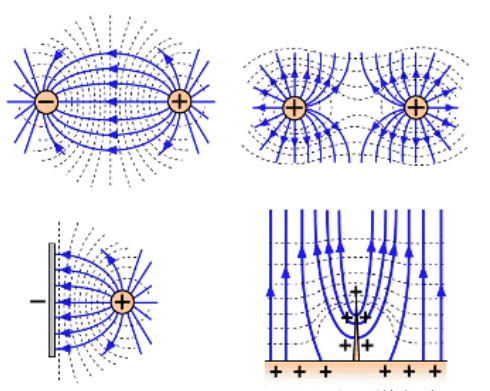
\includegraphics[scale=0.7]{1.png}
\end{center}
\textbf{Low Carbon Steel}
\begin{center}
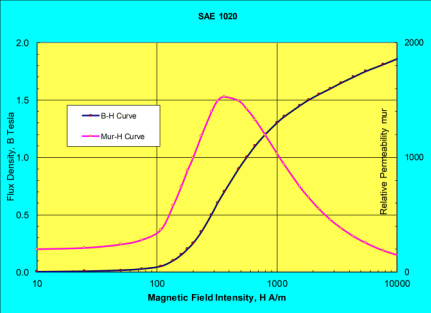
\includegraphics[scale=0.7]{2.png}
\end{center}
\newline
\textbf{Curie Temperature} refers to the temperature at which material loses its ferromagnetic properties and becomes paramagnetic.
\begin{itemize}
\item Fe - 770$^{\circ}$ C
\item Co - 1130$^{\circ}$ C
\end{itemize}
Samarium Cobalt (SmCo) is an example of high-temperature permanent magnets. SmCo is commonly found in electric propulsion systems since it operates at 300-500$^{\circ}$ C and has a Curie Temperature of 700$^{\circ}$ C.
\newline
\newline
\textbf{Relative Permeability}
\newline
\newline
We know from Equation 79 that,
\newline
\begin{equation*}
\begin{aligned}
\vv{B} = \mu_o \, (\vv{H}+\vv{M})
\end{aligned}
\end{equation*}
\newline
Substituting in the magnetic susceptibility (Equation 82), such that:
\newline
\begin{equation}
\begin{aligned}
\vv{B} = \mu_o \, (\vv{H}+\vv{M}) =\mu_o \, (\vv{H}+ \chi_m \, \vv{H}) = \mu_o \, (1 + \chi_m)\vv{H}
\end{aligned}
\end{equation}
\newline
We define \textbf{Permeability} (a material property) as
\newline
\begin{equation}
\begin{aligned}
\mu = \mu_o \, (1 + \chi_m)
\end{aligned}
\end{equation}
\newline
And (as we did with permittivity) we can define relative permeability as:
\newline
\begin{equation}
\begin{aligned}
K_m = \frac{\mu}{\mu_o} = 1 + \chi_m
\end{aligned}
\end{equation}
\newline

\newpage
\subsection{Boundary Conditions}

Similar to our Electrostatic Boundary Conditions, we can show that for a surface current density, $\vv{j}_s$ (Equation 71)
\newline
\begin{equation}
\begin{aligned}
(B_{\perp})_{2} = (B_{\perp})_{1}
\end{aligned}
\end{equation}
\newline
And from Equation 80
\begin{equation}
\begin{aligned}
(H_{||})_2 - (H_{||})_1 = \vv{j}_s \cdot \hat{n}
\end{aligned}
\end{equation}
\begin{center}
\vspace{100mm}
\textbf{Figure 21}
\end{center}
\newpage
\subsection{Magnetic Flux}
Magnetic flux is the flux through a given surface.
\newline
\begin{equation}
\begin{aligned}
\Phi _m = \int_S \vv{B} \cdot \hat{n} \, \mathrm{d}A \qquad \qquad  \big[\text{Webers}\big] = \big[T \cdot m^2\big]
\end{aligned}
\end{equation}
\newline
Note that flux through a closed surface is zero by Gauss's theorem
and the magnetic monopole law.
\newline
\begin{equation}
\begin{aligned}
\int_S \vv{B} \cdot \hat{n} \, \mathrm{d}A =  \int_{\volume} \nabla \cdot \vv{B} \, \mathrm{d}\volume =0
\end{aligned}
\end{equation}
\newline
\end{document}